 

The \emph{baseline} calibration (Sect.~\ref{se:baseline_calibration}) relies on
the \emph{baseline} scan selection, as defined in
Sect.~\ref{se:data_selection}, to mitigate the impact of
the \afternoon\ variation effect, as evidenced in Sect.~\ref{se:beam_variation}.
%,to focus as much as possible on pure on NIKA2 performances.
By contrast, in this section, we
address the issue of calibrating even during the observing periods
impacted by the \afternoon\ beam variation effect. We discuss an
alternative calibration method that
relies on a photometric correction depending on the beam size.
{\lp The key idea is to perform a joint monitoring of flux estimates
  using the fixed-width Gaussian amplitude and of the beam size.}
The objective is both to cross-check the baseline calibration results
using more observation scans and to anticipate on future developments
that could be deployed if an accurate beam monitoring is performed.

%We have however investigated alternative methods to correct for this effect
%(not related to the NIKA2 instrument)
%while extending the possible range of observing conditions. This section presents one
%of them, that relies on the monitoring of the effective FWHM during
%observations. It also offers and interesting cross-check of the baseline
%calibration.

\subsection{Photometric correction method}
\label{se:photometric_correction_method}

When the beam size broadens due to e.g. \afternoon\ beam effect, the flux
density is smeared in a larger solid angle and the flux density estimator, which
is based on the amplitude fit of a Gaussian beam of fixed FWHM (see
Sect.~\ref{se:photometric_system}) is biased towards low flux
densities.

Indeed, up to a normalization factor, the flux density
estimator in the reference photometric system (Sect.~\ref{se:photometric_system}) applied to a map
$M(\theta,\phi)$ reads

\begin{equation}
  \hat{S}  = \int \int M(\theta, \phi)\, e^{-\frac{d(\theta,\phi)^{2}}{2\sigma_{0}^{2}}} \sin \theta d\theta d\phi\,,
  \label{eq:flux_density_estimator}
\end{equation}

where $d(\theta,\phi)$ is the angular distance and $\sigma_0$
corresponds to FWHM$_0$
%, which we recall,
%is $12.5''$ for the $1\,\rm{mm}$ arrays and $18.5''$ for
%the $2\,\rm{mm}$ array
, as defined in Table~\ref{tab:definitions}.

Modelling the map of a point-like source with a single Gaussian of
width $\sigma$ and of amplitude $\mathcal{A}$ as

\begin{equation}
  M(\theta, \phi) = \mathcal{A} e^{-\frac{\theta^{2}}{2\sigma^2}}\,,
  \label{eq:pointsource_map}
\end{equation}

leads to

\begin{equation}
  \hat{S}  = 2\pi \sigma^2 \mathcal{A} \,  \frac{\sigma_0^2}{(\sigma^2 + \sigma_0^2)}.
  \label{eq:gaussian_star}
\end{equation}
As the map is calibrated using the reference Gaussian beam
(Sect.~\ref{se:photometric_system}), the absolute calibration factor %,
%which is evaluating as
%$S_{c}(\nu_{0})/\hat{S}_{c}$,
has a beam dependency that compensates the
$\sigma_0^2/(\sigma^2 + \sigma_0^2)$ factor in Eq.~\ref{eq:gaussian_star}.

Assume that we observe the source under stable conditions and
denote with a $\star$, the associated amplitude $\mathcal{A}_\star$, beam width
$\sigma_\star$ and flux estimate $\hat{S}_\star$. Using aperture
photometry, the energy conservation ensures that one has
$2\pi\sigma^2 \, \mathcal{A} = 2\pi\sigma_\star^2 \, \mathcal{A_\star}$.

To retrieve the flux estimate $\hat{S}_\star$ from the flux density
estimate $\hat{S}$, as obtained for any observations, a
corrected flux density $\hat{S}_{\rm{pc}}$ can be obtained using 
\begin{equation}
  \hat{S}_{\rm{pc}} = f(\sigma) \, \hat{S},
\end{equation} 
where the photometric correction is 
\begin{equation}
  f(\sigma) = \frac{(\sigma^2 + \sigma_0^2)}{(\sigma_\star^2+\sigma_0^2)}, 
\end{equation} 
so that $f(\sigma) = 1$ if $\sigma=\sigma_\star$.

%we can now derive the correct
%flux estimate $\hat{S}_\star$ from $\hat{S}$, as obtained under unstable conditions:
%
%\begin{equation}
%\hat{S}_\star = \frac{\sigma^2 + \sigma_0^2}{\sigma_\star^2 + \sigma_0^2}\hat{S}
%\equiv f(\sigma)\hat{S}.
%\end{equation}

Fig.~\ref{fig:f_sigma} shows how $f(\sigma)$ varies with the actual beam width
and for two choices of $\sigma_\star$ depending on the flux of the observed source.

\begin{figure}[ht!]
  \begin{center}
    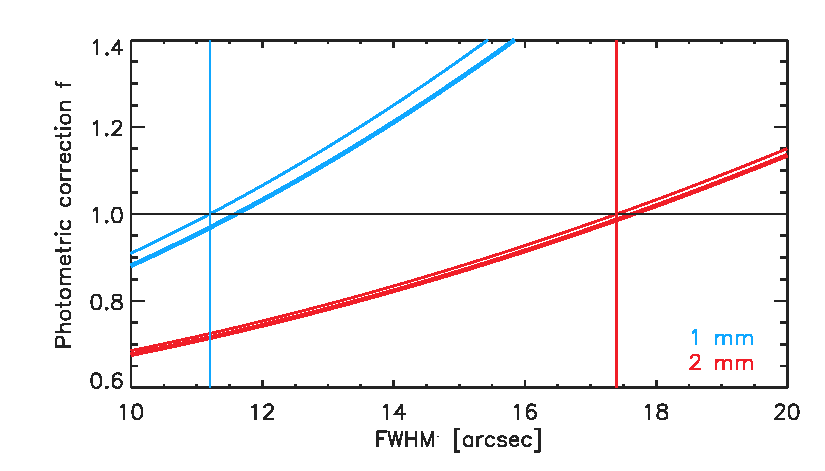
\includegraphics[clip=true, trim={0.9cm, 0.1cm, 0.5cm, 0.5cm}, width=0.4725\textwidth]{Figures/photometric_correction_function_1Jy.pdf}
    \caption[Photometric correction]{Magnitude of the beam photometric
      correction $f(\sigma)$ as a function of the actual FWHM, at 1\,mm (blue)
      and 2\,mm (red). Thick lines correspond to a choice of $\sigma_\star$
      derived on a very bright source like Uranus. Thin lines are for sources of
      1\,Jy at 1 and 2\,mm.}
\label{fig:f_sigma}
\end{center}
\end{figure}


%% Considering only the main beam broadening, modeled as a Gaussian of
%% size $FWHM = 2 \sqrt{2\ln{2}} \, \sigma$, we show in
%% Appendix~\ref{ap:photometric_correction_detail} that
%% the flux density estimator depends on {\lp $(\sigma'^2 +\sigma_0^2)$
%%   that is the squared size of the Gaussian
%%   resulting from the convolution} between the enlarged
%% $\sigma '$-Gaussian, which can be monitored as in Sect.~\ref{se:beam_variation}, and the 
%% $\sigma_0$ fixed-width Gaussian of our reference system.
%% 
%% An unbiased
%% flux density $\hat{S}_{\rm{pc}}$ can be derived from the flux density
%% estimate $\hat{S}$ as
%% \begin{equation}
%%   \hat{S}_{\rm{pc}} = f(\sigma')\, \hat{S},
%% \end{equation}
%% where $f(\sigma')$ is a photometric correction for the beam variation
%% effect. Within the Gaussian model, it reads:
%% \begin{equation}
%%   f(\sigma') = \frac{(\sigma'^2 + \sigma_0^2)}{(\sigma_{\star}^2 + \sigma_0^2)}. 
%% \end{equation} 

The beam size in stable atmospheric conditions $\sigma_\star$ is
determined by fitting the 2D Gaussian beam on the series of scans of
source with varying flux densities that have been used for the beam
characterization in Sect.~\ref{se:mainbeam}. However, $\sigma_\star$
is not equivalent to the main beam Gaussian size since the side lobes
and first error beams are not taken into account for this beam size
monitoring. The $\sigma_\star$ estimates are slightly
larger for bright sources due to the contribution of the first side
lobes and error beams, which are above the noise level, in the Gaussian fit.

%% An empirical model for the induced correlation of
%% $\sigma_\star$ with the source flux density is given in
%% Appendix~\ref{ap:photometric_correction_detail}.

\subsection{Monitoring of the temperature-induced beam size variation}
\label{ap:beam_monitoring}

The photometric correction thus relies on the measure of the current beam size
$\sigma$. The induced uncertainties on the flux density measurements depend on
the precision of the beam size determination. Here we
consider two methods to monitor the beam size.

The temperature-induced beam size variation is primarily monitored
using 2D Gaussian fit on all the available bright source observations,
as presented in Sect.~\ref{se:beam_variation}. 

For a finer sampling of the observation time, we also consider using
the pointing scans for beam monitoring. As discussed in
Sect.~\ref{se:pointing}, the telescope pointing is
monitored on a hourly basis during observation using {\tt pointing}
scans. As these scans consist of two sub-scans in azimuth and
elevation of about 10 seconds of integration time each, they
can also be used to make a map of the pointing source. For each campaign,
we thus have on hands hundreds of maps of mostly point-like bright
sources, which can also be used to monitor the beam size. 
%traitement pointing scans
For this purpose, {\tt pointing} scans are reduced 
and projected onto maps of $2''$ resolution using
the data analysis pipeline described in Sect.~\ref{se:dataproc}.
Fitting an elliptical 2D Gaussian to this map, we compute the geometrical FWHM.%$_{\rm{geom}}$
%is formed from the best-fit FWHM along the two axis.
%FWHM estimates on Uranus maps are corrected for an
%offset due to the finite size of the apparent disc, as discussed in
%Sect.~\ref{se:beam_monitoring_otf}.
{\tt Pointing} scans on {\lp slightly extended} sources, such as NGC7027,
are discarded from the analysis.

% anomalous refraction
For each {\tt pointing}, we also seek for signs of atmospheric
anomalous refraction. There are
enough KIDs per observation band to make an independent map using only
one subscan, i.e. 10 seconds of integration time.
For each of the four cross subscans, we thus estimate the position of the best
2D Gaussian that fits the map. We compute the deviation between each
subscan-derived position and the best-fit position using the entire
scan. An anomalous refraction event is detected when the difference is
above $2.5''$ for at least one subscan. We find that the \afternoon\
beam size variation effect is due to anomalous refraction for
between one third and one half of the scans, as reported in
Sect.~\ref{se:beam_variation}.

%\footnote{See the study posted
%  in the commissioning internal wiki at
%  \url{http://www.iram.fr/wiki/nika2/index.php/Millimetric_anomalies_(weather,_antenna)_as_monitored_by_pointing_scans}}.
%}   
The pointing-based FWHM estimates constitute a time-sampling of the
beam size during the whole observation campaign. They can serve to
estimate the beam size of any observation scans, in particular
towards sources too faint for a direct FWHM %$_{\rm{geom}}$
fit to be made on the map. However, we
expect less accuracy than using standard OTF raster
scans of bright sources due to the shorter integration time and the
fact that only the innermost KIDs in the array see the source.
To mitigate the dispersion, the time-stamped
pointing-based FWHM
%$_{\rm{geom}}$
is filtered with a running median on a 70-minute
width time window. Then, the FWHM %$_{\rm{geom}}$
at the time of the considered scans is
interpolated from the median-filtered pointing-based FWHM.%$_{\rm{geom}}$.
%
\begin{figure}[ht!]
  \begin{center}
    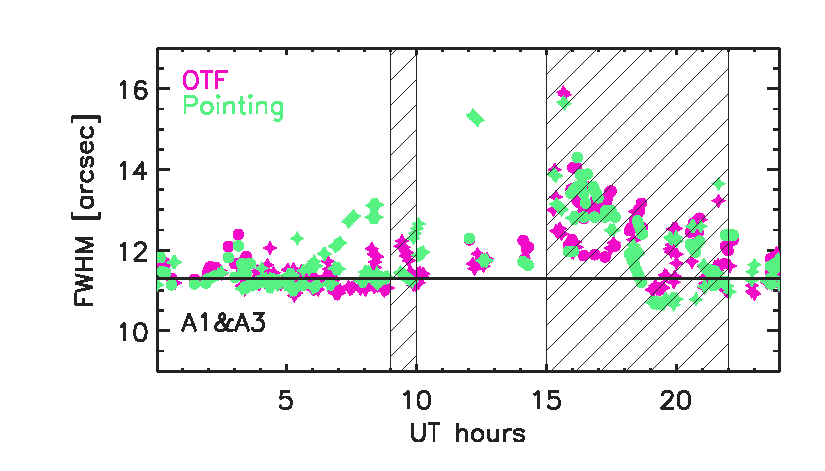
\includegraphics[clip=true, trim={0.9cm, 0.5cm, 0.5cm, 0.5cm}, width=0.4725\textwidth]{Figures/Beam_monitoring_with_otfs_vs_ut_compare_pointings_1mm.pdf}
    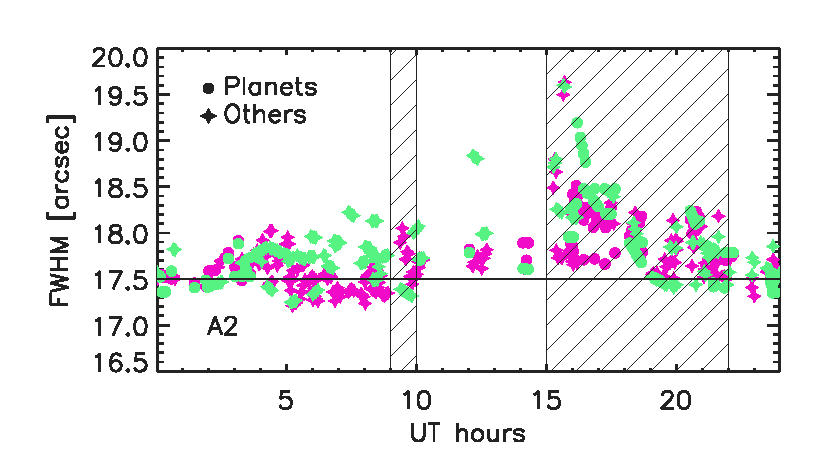
\includegraphics[clip=true, trim={0.5cm, 0.5cm, 0.5cm, 0.5cm}, width=0.4875\textwidth]{Figures/Beam_monitoring_with_otfs_vs_ut_compare_pointings_a2.pdf}
    \caption[Beam size monitoring comparison]{Beam size monitoring.
     'OTF'-labelled pink data points show the FWHM estimates from a 2D
    Gaussian fit on the maps of OTF raster scans towards bright
    sources, whereas the 'Pointing'-labelled light green data points
    are FWHM estimates obtained by interpolating the {\lp
    median-filtered} pointing-based FWHM at the time of the
    scans. {\lp The
    pointing-based FWHM estimates are obtained by fitting a 2D Gaussian on the
    maps of {\tt pointing} scans.}}
\label{fig:beam_monitoring_compare}
\end{center}
\end{figure}
%
Figure~\ref{fig:beam_monitoring_compare} shows two different FWHM %$_{\rm{geom}}$
estimates for the same data set: on one hand the best-fit FWHM %$_{\rm{geom}}$
estimates on the OTF-scan map and on the other hand the interpolation from
the pointing-based FWHM %$_{\rm{geom}}$
monitoring. The two estimates show the same global variations as a
function of the UT hours. They are well in agreement with each
other, although the pointing-based estimates have more dispersion and
a few outliers as expected.


\subsection{The two case studies}

We perform two case studies that correspond to the two beam monitoring
methods discussed above.\\
%\new{the paragraph titled ``Demonstration case''} presents a demonstration
%calibration assuming the beam is precisely monitored, whereas
%the ``Practical case using pointing scans'' paragraph addresses a practical calibration relying
%on a beam monitoring using pointing scans. 

\noindent \emph{Demonstration case} This method named {\tt PC-demo} hereafter, uses a
photometric correction based on the beam monitoring with bright source
scans. Both the 2D Gaussian FWHM fit and the FWHM$_0$ photometry are performed
on the map of the source. This method thus applies only to point-like sources
that are bright enough for an accurate fit of the beam on a single scan.

To capture only the beam size variations driven by the
observing conditions (primary mirror deformations, anomalous
refraction, elevation), a small correction $\delta_{\rm{FWHM}}$ has to be made to
the 2D Gaussian beam FWHM estimate for bright sources. The estimate of the
actual Gaussian size $\sigma$ is
\begin{equation}
  \hat{\sigma} = \frac{(\rm{FWHM} - \delta_{\rm{FWHM}})}{2\sqrt{2 \ln{2}}}, 
\end{equation} 
where the offset $\delta_{\rm{FWHM}}$ is null for faint or moderately
bright point sources, and non-zero for bright sources.
As for $\sigma_\star$, the 2D Gaussian fit yields slightly broader
FWHM for bright sources (e.g. planets) to accommodate
for the side lobes and error beams that are measured with high signal-to-noise.
For Uranus, $\delta_{\rm{FWHM}}$ includes also the beam widening due
to Uranus disc, as discussed in Sect.~\ref{se:mainbeam_results}.
%, which is seen with an average diameter of $3.5''$ at the
%IRAM 30-m telescope latitude.
We measure Uranus $\delta_{\rm{FWHM}}$
by comparing the average %$\sigma_{\rm{geom}}$
FWHM estimates using Uranus
scans and using MWC349 scans, we found $\delta_{\rm{FWHM}} = 0.4''$ at
1\,mm and $\delta_{\rm{FWHM}} = 0.25''$ at 2\,mm, which basically
distributes as one half being due to Uranus finite extension and the
other half stemming from the side lobes.\\

\noindent \emph{Practical case using pointing scans} This method,
named {\tt PC-point} hereafter, performs a photometric correction based on the beam monitoring with
pointing scans. 
%Indeed, pointing scans are performed on an hourly basis. They
%consist in two sub-scans in azimuth and elevation of about 10 seconds of
%integration time each, and provide high SNR on reference objects such as quasars
%or planets, hence good estimations of the
%FWHMs. Fig.~\ref{fig:beam_monitoring_compare} illustrates this point, by
%comparing the measured FWHM during pointing scans to standard OTF scans like in
%sect.~\ref{se:beam_variation}. We expect less accuracy though than with standard
%OTF raster scans of bright sources because of the shorter integration time. Both
%to mitigate the dispersion and to improve interpolations at any time, we use a
%running median filter of 70\,mn. {\tt Pointing} scans on {\lp slightly extended}
%sources, such as NGC7027, are discarded from the analysis. For each {\tt
%  pointing}, we also seek for signs of atmospheric anomalous refraction. There
%are enough KIDs per observation band to make an independent map using only one
%subscan, i.e. 10 seconds of integration time.  For each of the four cross
%subscans, we thus estimate the position of the best 2D Gaussian that fits the
%map. We compute the deviation between each subscan-derived position and the
%best-fit position using the entire scan. An anomalous refraction event is
%detected when the difference is above $2.5''$ for at least one subscan. We find
%that the apparent beam broadening during the afternoon is due to anomalous
%refraction for between one third and one half of the scans over the period
%studied here.
Unlike {\tt PC-demo}, this method is usable even for sources fainter than
about one Jy \nico{but relies on interpolations between beam width estimates on
  other scans}. For Uranus, this value is corrected for the diameter size, as in
Sect.~\ref{se:mainbeam_results}. No other FWHM offset correction is needed since
pointing scan maps have a low signal-to-noise ratio that prevents the
geometrical FWHM from being significantly affected by the side lobes.


\subsection{Absolute calibration with a photometric correction}

We perform the absolute calibration by i) implementing the reference
method described in Sect.~\ref{se:practical_calib}, ii) correcting the
atmospheric attenuation using the {\tt corrected skydip} opacity
estimates, and iii) using the photometric correction of
Appendix~\ref{se:photometric_correction_method}.


%%%%%%%%%%%%%%%%%%%%%%%%%%%%%%%%%%%%%%%%%%%%%%%%%%%%%%%%%%%%%%%%%%%
%    Flux ratio vs FWHM
\begin{figure}[!htbp]
  \begin{center}
    % corr. sky. photocorr demo
    \begin{overpic}[clip=true, trim={0, -0.3cm, -0.3cm, 0},width=0.525\linewidth]{Figures/plot_flux_density_ratio_fwhm_uranus_corrected_skydip_photocorr_demo_narrow_1mm.pdf}
       \put(18,25){\footnotesize PC-demo}
    \end{overpic}
    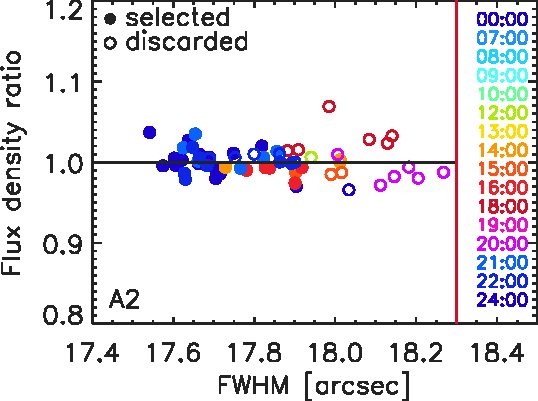
\includegraphics[clip=true, trim={0.7cm, -0.3cm, -0.25cm, 0}, width=0.465\linewidth]{Figures/plot_flux_density_ratio_fwhm_uranus_corrected_skydip_photocorr_demo_narrow_a2.pdf}
    % corr. sky. photocorr pointing
    \begin{overpic}[clip=true, trim={0, -0.3cm, -0.3cm, 0},width=0.525\linewidth]{Figures/plot_flux_density_ratio_fwhm_uranus_corrected_skydip_photocorr_pointing_narrow_1mm.pdf}
      \put(18,25){\footnotesize PC-point}
    \end{overpic}
    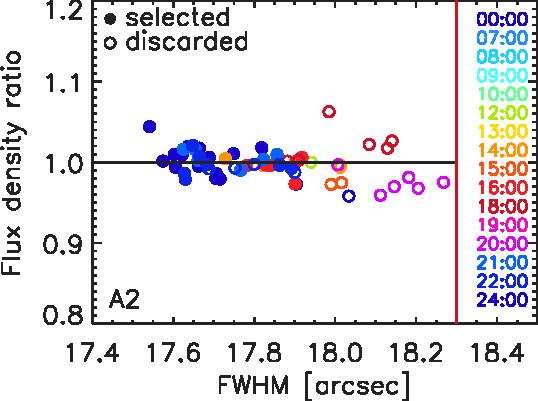
\includegraphics[clip=true, trim={0.7cm, -0.3cm, -0.25cm, 0}, width=0.465\linewidth]{Figures/plot_flux_density_ratio_fwhm_uranus_corrected_skydip_photocorr_pointing_narrow_a2.pdf}
    \vspace{-0.5cm}
    \caption[Uranus flux density stability against FWHM]{
      \small{Uranus flux density ratio vs beam size for calibration
  with photometric correction. The ratio of 
      Uranus measured flux densities to expectations as a function of the
      measured 2D Gaussian beam FWHM is shown for the $1$-mm array
      combination (left column) and for array 2 (right column) after absolute
      calibration using (\emph{first row}) the {\tt PC-demo} and (\emph{second
        row}) the {\tt PC-point} photometric corrections. These plots
      include all Uranus scans acquired during N2R9, N2R12 and N2R14
      campaigns and whose beam FWHMs are below the threshold indicated
      by the vertical red lines, (open circles), as
      well as the scans that met the baseline scan selection criteria (filled
      circles). 38 scans now pass the \emph{baseline} selection criteria vs 26
      only without photometric correction (see also Fig.~\ref{fig:calib_uranus_vs_fwhm_all}).}}
\label{fig:calib_uranus_vs_fwhm_photocorr}
\end{center}
\end{figure}

Using the photometric correction alleviates the need of
performing a scan selection based on the observation time. However,
the scans from which the absolute calibration is derived, are selected
on the FWHM estimate using the same criteria as for the baseline
calibration, that are FWHM thresholds of $12.5''$ at $1\, \rm{mm}$ and $18''$ at
$2\, \rm{mm}$. Thus, only the scans that are moderately affected by the beam
effect are included in the absolute calibration in order not to
include twice the photometric correction uncertainties in the error
budget (once for the absolute calibration and once for the photometry).

Figure~\ref{fig:calib_uranus_vs_fwhm_photocorr} presents the Uranus
measured-to-predicted flux density ratio as a function of the beam FWHM
after the photometric correction with the {\tt PC-demo} and
{\tt PC-point} methods. The flux
density is stable against the beam FWHM within uncertainties for both
wavelengths.

% ALL METHOD RESULTS 
\begin{table}[!htbp]
\caption[Comparison of calibration results using five methods]{Comparison of absolute calibration results using five methods}
\label{tab:Abs_calibration_results_all}
\centering
\begin{tabular}{clrrrrr}
  \hline\hline
  \noalign{\smallskip}
%  \multicolumn{2}{c}{}  &  \multicolumn{5}{|c|}{Methods} \\\cline{3-7}
  \multicolumn{2}{c}{}  &  baseline  & TM\tablefootmark{a}  &  SD\tablefootmark{b} & PC-d\tablefootmark{c} & PC-p\tablefootmark{d}  \\
  \noalign{\smallskip}
  \hline\hline
   \multicolumn{2}{c}{$\#$ scans} & 26    &       26  &    26    &    38           &    38 \\ 
  \hline
  \noalign{\smallskip}
%  Factor &  A1          &   1.00  &  0.97   &  1.13    &   1.01    &   1.02  \\
%         &  A3          &   1.00  &  0.97   &  1.02    &   1.01    &   1.00  \\
   Ratio  &  1mm         &   1.00  &  0.95   &  1.06    &   1.01    &   1.01  \\
          &  2mm         &   1.00  &  0.94   &  0.99    &   1.01    &   1.01  \\
  \hline
  \noalign{\smallskip}
%  RMS  &  A1            &  3.2    &   4.2   &   3.4    &    3.5    &   3.0 \\
%  $[\%]$     &  A3      &  3.6    &   4.3   &   3.3    &    3.5    &   3.0 \\
   RMS    &  1mm           &  3.3    &   4.5   &   3.3    &    3.1    &   2.6 \\
   $[\%]$ &  2mm           &  1.6    &   2.6   &   1.5    &    1.5    &   1.5 \\
\hline
\end{tabular}
\tablefoot{ Results based on 
    \tablefoottext{a}{the {\tt Taumeter} opacity correction}
    \tablefoottext{b}{the {\tt Skydip} opacity correction}
    \tablefoottext{c}{the {\tt PC-demo} photometry correction}
    \tablefoottext{d}{the {\tt PC-point} photometry correction}
    }
\end{table}

We further quantify the
difference between all the calibration methods that have been tested
in evaluating i) the average absolute calibration factor
with respect to the baseline calibration factor and
ii) the rms dispersion of the measured-to-modelled flux ratios. These
quantities are gathered in Table~\ref{tab:Abs_calibration_results_all}
in the rows labelled 'Ratio' and 'RMS' respectively. 

We find that, resorting to a photometric correction i) allows us to use $45\%$ more
scans for the absolute calibration, ii) has a negligible impact on
the absolute calibration factor and iii) yields a small reduction of
the flux density ratio dispersion. For the absolute calibration, the
{\tt PC-point} method performs as well as the {\tt PC-demo} one.
Photometry capability and stability when using a photometric
correction are further tested in Sect.~\ref{se:photometry}.\\


%% % flux-dependency of sigma stable
%% \begin{figure}[ht!]
%%   \begin{center}
%%     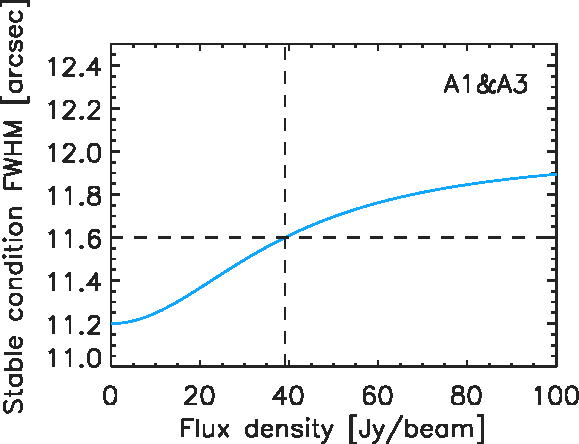
\includegraphics[clip=true, trim={0, -0.3cm, -0.3cm, 0}, width=0.49\linewidth]{Figures/FWHM_stable_empiric_ref_1mm.pdf}
%%     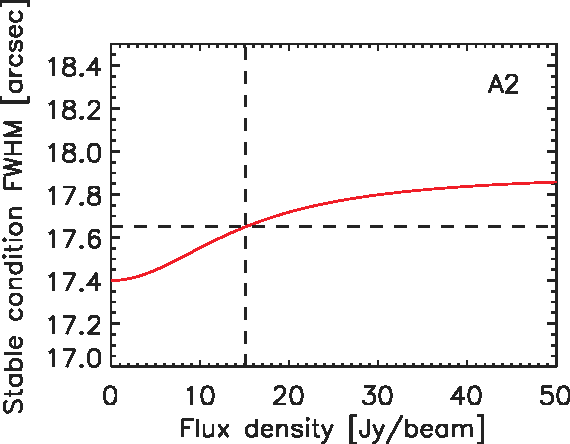
\includegraphics[clip=true, trim={0, -0.3cm, -0.3cm, 0}, width=0.49\linewidth]{Figures/FWHM_stable_empiric_ref_a2.pdf}
%%     \caption[Photometric correction pivot Gaussian
%%       size]{Flux-dependency of the pivot size $\sigma_\star$ of the
%%       Gaussian beam used for the photometric correction. %This is measured as the 2D
%%       %Gaussian fit of the map observed in stable conditions.
%%       The vertical dashed lines correspond to Uranus flux densities in
%%       the two bands, and the horizontal dashed lines are the FWHMs
%%     corresponding to the measured $\sigma_\star$ towards Uranus.}
%%     \label{fig:sigma_stable_vs_flux}
%%   \end{center}
%% \end{figure}

%% As discussed in Sect.~\ref{se:beam_variation}, the beam size is
%% monitored by fitting a 2D Gaussian of freely varying FWHM.
%% %In practice,
%% %the pivot Gaussian size $\sigma_{\star}$ thus corresponds
%% %to the nominal size of the 2D Gaussian fit of the beam that is
%% %measured in stable observing conditions.
%% We find the Gaussian size $\sigma_{\star}$ slightly varies with the
%% source flux density. Whereas it basically corresponds to the main beam
%% size for faint to moderately bright point sources, it is slightly
%% larger for bright sources. The simple 2D Gaussian fit
%% accomodates with the more complex beam pattern features that are well
%% above the noise level (see Sect.~\ref{se:fullbeam}) in the case of
%% bright sources.
%% %bright enough for the side lobes to be well above the noise level.
%% %The variation of $\sigma_{\star}$ can be seen as a
%% %correction for fitting the complex beam pattern, as presented in
%% %Sect.~\ref{se:fullbeam}, with a single 2D Gaussian of freely varying
%% %size.
%% 
%% In Fig.~\ref{fig:sigma_stable_vs_flux}, we give an
%% empirical model for the flux dependency of the FWHM derived from
%% $\sigma_{\star}$: it
%% smoothly goes from $11.2''$ at $1\,\rm{mm}$ and $17.4''$ at $2\,\rm{mm}$ for
%% faint sources to $11.6''$ at $1\,\rm{mm}$ and $17.65''$ at
%% $2\,\rm{mm}$ at the flux density of Uranus,
%% then slightly continues increasing for sources brighter than Uranus.


%% \subsubsection{Beam monitoring using pointing}
%% \label{se:beam_monitoring_pointing}
%% 
%% For a finer sampling of the observation time, we also consider using the
%% pointing scans for beam monitoring. As discussed in Sect.~\ref{se:pointing}, the
%% telescope pointing is monitored on a hour basis during observation using {\tt
%%   pointing} scans. As these scans consist of two sub-scans in azimuth and
%% elevation of about 10 seconds of integration time each, they can also be used to
%% make a map of the pointing source. For each campaign, we thus have hundreds of
%% maps of mostly point-like bright sources in hands, that can also be used to
%% monitor the beam size. Fig.~\ref{fig:beam_monitoring_compare} illustrates this
%% point, by comparing the measured FWHM during pointing scans to standard OTF
%% scans like in sect.~\ref{se:beam_variation}. We expect less accuracy though than
%% with standard OTF raster scans of bright sources because of the shorter integration
%% time. Both to mitigate the dispersion and to improve interpolations at any
%% time, we use a running median filter of 70\,mn. {\tt Pointing} scans
%% on {\lp slightly extended} sources, such as NGC7027, are discarded from the
%% analysis.
%% 
%% % anomalous refraction
%% For each {\tt pointing}, we also seek for signs of atmospheric anomalous refraction. There are
%% enough KIDs per observation band to make an independent map using only
%% one subscan, i.e. 10 seconds of integration time.
%% For each of the four cross subscans, we thus estimate the position of the best
%% 2D Gaussian that fits the map. We compute the deviation between each
%% subscan-derived position and the best-fit position using the entire
%% scan. An anomalous refraction event is detected when the difference is
%% above $2.5''$ for at least one subscan. We find that the apparent beam
%% broadening during the afternoon is due to anomalous refraction for
%% between one third and one half of the scans over the period studied
%% here.
%% %\footnote{See the study posted
%% %  in the commissioning internal wiki at
%% %  \url{http://www.iram.fr/wiki/nika2/index.php/Millimetric_anomalies_(weather,_antenna)_as_monitored_by_pointing_scans}}.
%% %} 
%% 
%% %In Fig.~\ref{fig:beam_monitoring_pointing}, we present the FWHM
%% %estimates using pointing scans as a function of the observing time in
%% %UT hours for three observation campaigns. We observe the same beam
%% %size evolution with UT hours as previously discussed in
%% %Sect.~\ref{se:beam_monitoring_otf}, that is a plateau during night-time
%% %and a smooth increase during day-time up to a maximum in the
%% %afternoon, which is followed by a smooth decrease down to the plateau
%% %a few hours after the sunset. Although the general trend is the same
%% %as the OTF-based FWHM variations, more dispersion is seen either using
%% %pointings toward giant planets or other bright sources.
%% %
%% %\begin{figure}[ht!]
%% %  \begin{center}
%% %    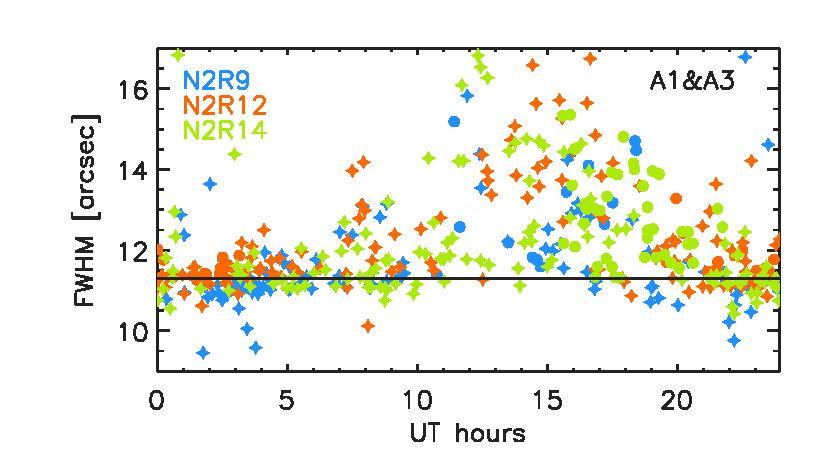
\includegraphics[clip=true, trim={0.9cm, 0.5cm, 0.5cm, 0.5cm}, width=0.4725\textwidth]{Figures/Beams/Beam_monitoring_with_pointings_vs_ut_1mm.pdf}
%% %    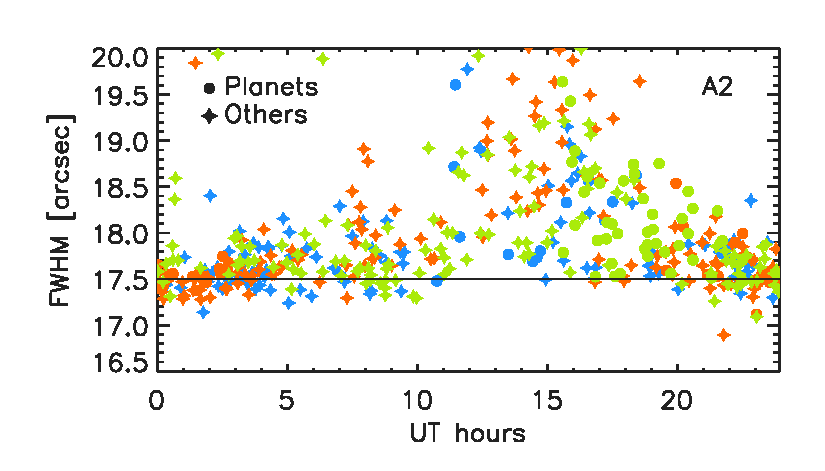
\includegraphics[clip=true, trim={0.5cm, 0.5cm, 0.5cm, 0.5cm}, width=0.4875\textwidth]{Figures/Beams/Beam_monitoring_with_pointings_vs_ut_a2.pdf}
%% %    \caption[Beam size monitoring using pointing scans]{Beam size
%% %      monitoring using pointing scans. Same legend as in
%% %      Fig.~\ref{fig:beam_monitoring_otf}.} 
%% %\label{fig:beam_monitoring_pointing}
%% %\end{center}
%% %\end{figure}
%% %
%% %% The pointing-based FWHM estimates constitute a time-sampling of the
%% %% beam size during
%% %% the whole observation campaign. They can serve to estimate the beam
%% %% size of any observation scans, in particular
%% %% toward sources too faint for a direct FWHM %$_{\rm{geom}}$
%% %% fit to be made on the map. To mitigate the dispersion, the time-stamped
%% %% pointing-based FWHM
%% %% %$_{\rm{geom}}$
%% %% is filtered with a running median on a 70-minute
%% %% width time window. Then, the FWHM %$_{\rm{geom}}$
%% %% at the time of the considered scans is
%% %% interpolated from the median-filtered pointing-based FWHM.%$_{\rm{geom}}$.
%% %% %
%% \begin{figure}[ht!]
%%   \begin{center}
%%     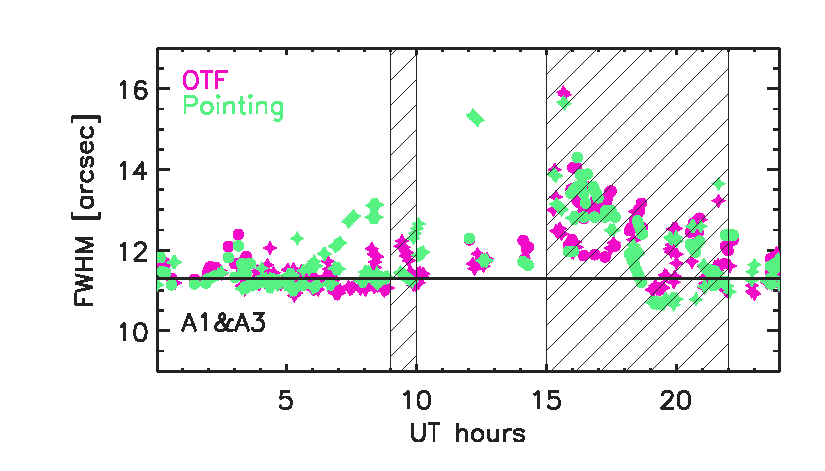
\includegraphics[clip=true, trim={0.9cm, 0.5cm, 0.5cm, 0.5cm}, width=0.4725\textwidth]{Figures/Beam_monitoring_with_otfs_vs_ut_compare_pointings_1mm.pdf}
%%     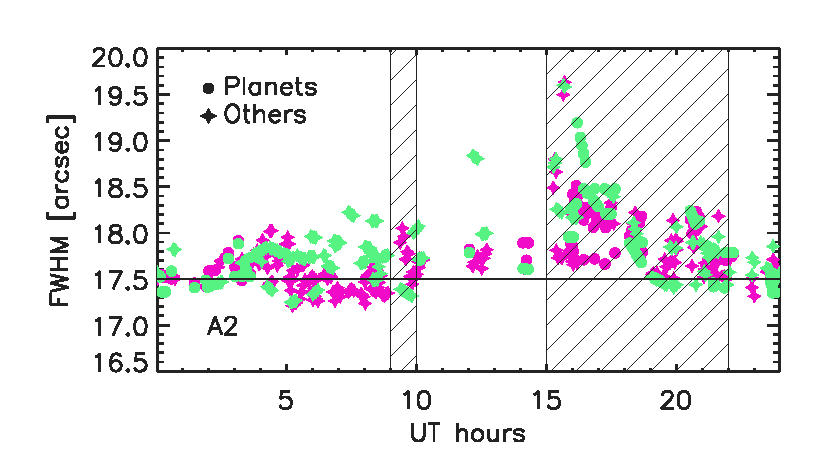
\includegraphics[clip=true, trim={0.5cm, 0.5cm, 0.5cm, 0.5cm}, width=0.4875\textwidth]{Figures/Beam_monitoring_with_otfs_vs_ut_compare_pointings_a2.pdf}
%%     \caption[Beam size monitoring comparison]{Beam size monitoring.
%%      'OTF'-labeled pink data points show the FWHM estimates from a 2D
%%     Gaussian fit on the maps of OTF raster scans towards bright
%%     sources, whereas the 'Pointing'-labeled light green data points
%%     are FWHM estimates obtained by interpolating the {\lp
%%     median-filtered} pointing-based FWHM at the time of the
%%     scans. {\lp The
%%     pointing-based FWHM estimates are obtained by fitting a 2D Gaussian on the
%%     maps of {\tt pointing} scans.}}
%% \label{fig:beam_monitoring_compare}
%% \end{center}
%% \end{figure}
%% %% %
%% %% Figure~\ref{fig:beam_monitoring_compare} shows two different FWHM %$_{\rm{geom}}$
%% %% estimates for the same data set: on one hand the best-fit FWHM %$_{\rm{geom}}$
%% %% estimates on the OTF-scan map and on the other hand the interpolation from
%% %% the pointing-based FWHM %$_{\rm{geom}}$
%% %% monitoring. The two estimates show the same global variations as a
%% %% function of the UT hours. They are well in agreement with each
%% %% other, although the pointing-based estimates have more dispersion and
%% %% a few outliers.
